\chapter{Background and Motivation}
\label{backgrnd}
\quad \textit{Parallel computing} and \textit{software parallelization} are vast, overlapping and complementary computer science areas with a history dating back to 1950s. With the advances in semiconductor industry the topics have left the niche of high-end scientific supercomputers and spread to a much wider area spanning across all consumer electronic devices and have become of major importance.\newline\null
% Parallel computing and software parallelization are vast, complementary and overlapping areas omnipresent across the whole spectrum of hardware. The topics of major importance.
\quad Nowadays parallelism is pervasive. Parallel hardware is omnipresent across the whole wide spectrum of computing systems. In order to exploit all the available hardware capabilities software has to be parallel as well. And thus, every computer scientist and software developer would benefit from having an insight into the area. Nonetheless, the topics are extremely difficult, require a serious time investment and a great deal of knowledge in various subdomains. It is not always realistic to expect an average programmer to possess such a deep expertise. For that reason we propose a solution aimed at alleviating the challenging task of manual software parallelization. Our solution consists of the two components. We describe them in Chapters \ref{assistant} and \ref{frameworks}.\newline\null
% Background chapter as the point of basic material accumulation. Based on LLNL tutorials!
\quad In this chapter we accumulate and structure the material, which stresses the importance of software parallelization, highlights its challenges, describes the parallel software engineering process and finally lays the ground for our proposed solutions from Chapters \ref{assistant} and \ref{frameworks}. \textbf{The major ideas leading towards the solutions from Chapters \ref{assistant} and \ref{frameworks} are highlighted with bold face text.} We express our special gratitude to Lawrence Livermore National Laboratory (LLNL) \cite{llnl_computing} for their great parallel computing tutorials. We heavily relied on those to prepare the material of this chapter.\newline\null
% The story line:
%
% Parallel computing importance
% Challenges of software parallelization:
%     automatic
%     manual
%     machine learning based
%     data-centric parallelization problem
% 
%
\quad The background chapter is structured as follows. Section \ref{background_importance} stresses the importance of parallel computing and software parallelization in the modern world. There are numerous software parallelization methods and techniques, but all of them run into their specific challenges and problems. Section \ref{background_challenges} highlights the major problems of various software parallelisation methods. First, it presents the challenges of manual and then automatic software parallelization techniques. There have been various experiments and works employing machine learning (ML) based methods \cite{ml-oboyle} for the task of software parallelization. These challenges form the ground for our program loop parallelization assistant solution \cite{assistant-aiseps} to grow on. We describe our solution in Chapter \ref{assistant}. Then, in Section \ref{background_dcp} we discuss the problem of data structure choice and how it affects the software parallelization. In Section \ref{background_dcp_literature_review} we present a thorough literature review on the topic of Data Centric Parallelization (DCP) dealing with the task of automatic data structure recognition. Our review concludes with an observation that an automatic data structure recognition techniques are still an unsolved grand challenge. Data structures are often inseparable from the algorithms they support. Our computational frameworks build on that fact by defining the blend of data structures and algorithms. We propose our solution to the problem in Chapter \ref{frameworks}. Furthermore, modern software design and engineering tasks are extremely rich and complex topics. That is true of parallel software engineering as well of course. In Sections \ref{background_programming_paradigms} and \ref{background_oop_design} we talk about imperative, functional and object-oriented programming paradigms, as well as various OOP software design patterns. Our computational frameworks take the best from these principles and alleviate the task of parallel software architecture design for an average programmer.
\section{The importance of parallel computing}
\label{backgrnd_importance}
\quad Parallelism is pervasive and the future of computing is parallel. There are many factors which stress the importance of parallelism in the modern computing world.
\begin{description}[style=unboxed,leftmargin=0cm]
\itemsep0em
\item[Abundance of natural parallelism] The field of High Performance Computing (HPC) has traditionally been concerned with scientific modelling and simulation of various natural phenomena (climate change, fluid flows, etc.). Such systems consist of numerous often independent parts. When we compile a highly parallel algorithm to a serial sequence of CPU instructions or process a huge data set with independent parts sequentially we are artificially constraining a vastly parallel computation to a serial one. Parallelism is not limited by the natural world, instead many algorithms have inherent parallelism in them.
\item[Semiconductor technology advances and power limits] With advances in transistor density it became feasible to design more complicated CPUs. Initially the trend went into complex microarchitecture, for example, deeper pipelines, but running into power limits the industry design shifted towards multi core CPUs and multiprocessor systems. Such systems require of software to mirror the trend and become parallel as well.
\item[Domain inherent parallelism and specialized computations] The areas like computer graphics for instance have a lot of problems that can be processed in a Single Instruction Multiple Data (SIMD) fashion. That naturally led to specialized co-processors like GPUs. Hardware systems become more complex and heterogeneous now.
\end{description}
\section{Challenges in software parallelization}
\label{backgrnd_challenges}
\quad The problem of software parallelization is extremely complex and multi-faceted. There are various approaches to the problem, but all of them have their pros and cons. Although, the process of software parallelization has characteristically been a very \textit{manual} task, which is time-consuming and error-prone, there are also \textit{automatic} and \textit{machine learning based} techniques. In this section we highlight inherent challenges of these approaches. The solution we propose aims to alleviate these.
\subsection{Manual parallelization challenges}
\label{background_challenges_manual}
\quad Parallel software development has characteristically been a very manual process. As any software development process it consists of a number of stages and parts. The major problems are described below.
\begin{description}[style=unboxed,leftmargin=0cm]
\itemsep0em
\item[Problem understanding and partitioning] As the best software engineering practices dictate, before diving into software development one needs to thoroughly understand the problem and decide on the requirements and restrictions the final piece of software must meet. The whole algorithm and software architecture might change with the decision of developing a parallel software version instead of a serial one. If one starts from an already implemented serial software version, the parallelization might be even more difficult to do. Source code comprehension is a hard task. The algorithm chosen for a serial version might be completely unsuitable for a parallel implementation. The problem must be partitioned into relatively independent chunks of work to be processed in parallel. The partitioning can be done in numerous ways and a programmer needs to choose the way to do that (data set decomposition, functional decomposition or a hybrid of the two).
\item[Communications and synchronization] Very often the parts of the problem are not completely independent and require an exchange of information. Designing the way that exchange is going to work is a complex task. Almost always communication results in an overhead. Sending the data over congested network or waiting on a synchronization barrier slows the program down. The slowdown might even diminish all performance benefits obtained from parallelization.
\item[Implementation and data dependencies] When the problem partitioning is done, all communication and synchronization points are determined and the high level parallel algorithm is designed, a programmer might start the actual implementation. Here a programmer will run into other types of problems. Consider two functionally equivalent code samples below.\newline\null
\begin{minipage}[t]{0.50\linewidth}
\begin{lstlisting}[caption={\raggedright Non-parallelizable loop with planted loop-carried data dependence.},label={lst:code_sample_data_dependence},language=C]
for (int i=1; i<n; i++) {
  a[i]=a[i-1]+1;
}
\end{lstlisting}
\end{minipage}
\begin{minipage}[t]{0.50\linewidth}
\begin{lstlisting}[caption={\raggedright Parallelizable loop free of any data dependencies.}, label={lst:code_sample_no_data_dependence},language=C]
for (int i=0; i<n; i++) {
  a[i]=a[0]+i;
}
\end{lstlisting}
\end{minipage}

The actual shape of the code can break parallelization by introducing fake (not required by the algorithm) dependencies.
\item[Performance analysis and tuning] One needs to know where the program's hotspots are. Hotspots are the places where the most of the real work is being done. The majority of programs spend most of the CPU time in a few places. The task of a programmer is to find those places and concentrate all parallelization and optimization efforts right there. Finding hotspots might be difficult before the programmer has the whole program implemented. Modern hardware architectures have a multi level memory hierarchy, memory data prefetchers, TLBs, out-of-order execution, etc. It might be surprising how the actual program execution performance differs from the one inferred from the algorithm. Profilers and other analysis tools can be of help here.
\end{description}
\quad Finally, all the above challenges are interrelated and very often depend on each other. The parallel software development process can go iteratively with numerous dead ends and redesign efforts. With a long research history into the topic, all these problems are still actual now.
\subsection{Limitations of automatic techniques}
\label{backgrnd_challenges_automatic}
\quad Given the enormous challenges of manual software parallelization there have been numerous attempts to automate the task. There are various tools available to assist a programmer in the task of software parallelization. Parallelizing compilers \cite{llvm-compiler-infrastructure}\cite{icc-compiler} are the most widely used. Below we present their classification:
\begin{description}[style=unboxed,leftmargin=0cm,noitemsep]
\itemsep0em
\item[Fully Automatic] The compiler analyzes the source code and identifies opportunities for parallelisation. The analysis includes identifying inhibitors to parallelism and possibly a cost weighting on whether or not the parallelisation would actually improve performance \cite{Kennedy:2001:OCM:502981}. Loops are the most frequent target for automatic parallelization \cite{Bacon:1994:CTH:197405.197406}.
\item[Programmer Directed] Using compiler directives or possibly compiler flags, a programmer explicitly tells the compiler how to parallelize the code. These directives and flags may be also used in conjunction with some degree of automatic parallelization. The most common compiler generated parallelization is done using on-node shared memory and threads (such as OpenMP \cite{Dagum:1998:OIA:615255.615542}).
\end{description}
\quad If one is starting with an existing serial code and has time or budget constraints, then automatic parallelization may be the answer. However, there are several important caveats that apply to automatic parallelization.
\begin{description}[style=unboxed,leftmargin=0cm]
\itemsep0em
\item[Performance] Performance may actually degrade.
\item[Limitations] Limited to a subset (mostly loops) of code.
\item[Effectiveness] May actually not parallelize code i.e. it may be "over conservative" or the code is too complex.
\end{description}
\quad To clearly illustrate the problems an automatic software parallelization faces we conducted several experiments with the suite of NASA Parallel Benchmarks (NPB) \cite{nasa-parallel-benchmarks}. These benchmarks target performance evaluation of highly parallel supercomputers. Consequently, the suite has a great amount of inherent parallelism and is supposed to be relatively easy parallelizable. NPB benchmarks do not provide the exact implementation, they rather specify what should be computed and how. We used Seoul National University's (SNU) implementation \cite{snu-npb-benchmarks} of NPB benchmarks. SNU NPB implementation comes in two versions: sequential legacy C implementation and the one parallelized with OpenMP pragmas. The main data structure used everywhere in the suite is a simple flat array. There are numerous loop nests operating over arrays and computing simple reductions.\newline\null
\quad For these experiments we used a desktop Ubuntu 18.04 machine with installed Intel C/C++ Compiler (ICC) 18.0 and measured the running time of benchmarks with the help of UNIX time() utility. To minimize the errors, we ran experiments several times and took the mean average. The machine has 4 Intel Core i5-6500 CPUs with 3.20 GHz frequency and vectorization support up to AVX2. The RAM is 16Gb.\newline\null
\quad The first experiment we conducted was aimed at assessing the effectiveness of the state-of-the-art automatic parallelization. The experiment is platform agnostic as long as the target supports vector instructions and parallel primitives and can be reproduced on any such platform. We took the Intel C/C++ Compiler (ICC), configured it for the most aggressive parallelization (\textit{-par-threshold0}), i.e parallelize all parallelizable code independent of its potential cost weighted profitability. Also, we configured ICC to do all enabling loop transformations (\textit{-O3} flag) before the actual parallelization (\textit{-parallel} flag) and vertorization (\textit{-vector} flag). In other words, the experiment measures the maximum parallelization coverage the best state-of-the-art compiler can have on embarrassingly parallel problems, which still represent the real world code. Our results show a significant potential for improvement. Among all 1415 SNU NPB loops, 980 are truly parallelizable, but the ICC compiler manages to find only 812 parallelizable cases and misses 168 loops. Table \ref{tab:icc_missed} shows the classification we conducted by manually examining the ICC parallelization reports as well as looking at the source code of the benchmarks. The biggest problems are statically unknown pointers, which might potentially overlap at the running time, as well as other statically unresolvable dependencies. There are some unrecognized reductions as well as loops that can be parallelized with prior array privatization and function inlining.
\begin{table}
  \begin{minipage}{\pagewidth}
  \begin{center}
    \begin{tabu}{M{3.0cm}M{1.0cm}M{3.0cm}M{1.0cm}M{3.0cm}M{1.0cm}}
      \hline
      \rowfont{\bfseries}
      reason & num & reason & num & reason & num\\\hline
      \textbf{unrecognised reduction} & 18 & \textbf{array privatization} & 7 & \textbf{AA conservativeness} & 60\\\hline
      \textbf{unknown iteration number} & 7 & \textbf{static dependencies} & 46 & \textbf{too complex} & 22\\\hline
      \textbf{uninlined calls} & 4 & \textbf{other} & 4 & \textbf{total} & 168\\\hline
    \end{tabu}
  \end{center}
  \end{minipage}
  \caption{Classification of loops missed by Intel Compiler for various reasons.}
  \label{tab:icc_missed}
\end{table}\newline\null
\quad While parallelization coverage is important it is not the primary goal. A parallelized loop might not make a significant contribution to the total running time of the application. We should strive to parallelize those loops, which are on the critical paths and hot spots. And finally, only the running time is the ultimate parallelization performance measure. Given that, we conducted a further experiment. We used the same machine and compiled SNU NPB benchmarks with different sets of ICC automatic parallelization options. Figure \ref{fig:benchmarks_runtime} illustrates the running times of resulting codes. Bars marked as serial (s) show running times of original legacy C sequential versions. Bars marked as omp (o) show running times of an expertly manually parallelized versions. Other bars show running times of versions produced with various combinations of ICC compiler options (vectorize, parallelize or do both), as well as complete cases of parallel OpenMP versions, which have been additionally parallelized and vectorized by the ICC compiler. One can see that the best performance is still attributed to benchmark versions, which have been expertly parallelizad by their developers. Vectorization and parallelization help parallel versions a bit, but not that significantly and the profits can be neglected altogether. When we automatically vectorize serial versions we get a little improvement, but when we try to automatically parallelize them we get striking slowdowns on some benchmarks. Overall, automatic vectorization gives us a tiny 1.1x running time improvement in the geometric mean compared to 1.73x of manual parallelization. And the automatic parallelization results into 0.79x slowdown in the geometric mean across all the benchmarks.\newline\null
\textbf{\quad Our machine learning based loop parallelization assistant \cite{assistant-aiseps} we propose in Chapter \ref{assistant} extends parallelism recognition capabilities of the Intel C/C++ Compiler (ICC) by learning the loop parallelizability property and making predictions regarding it with an acceptable false positives rate. These predictions cover most of the cases missed by ICC. Moreover, our assistant helps to reach the best possible manual expert performance faster by guiding the programmer towards to the most fruitful code segments to parallelize.}
\begin{figure}[ht]
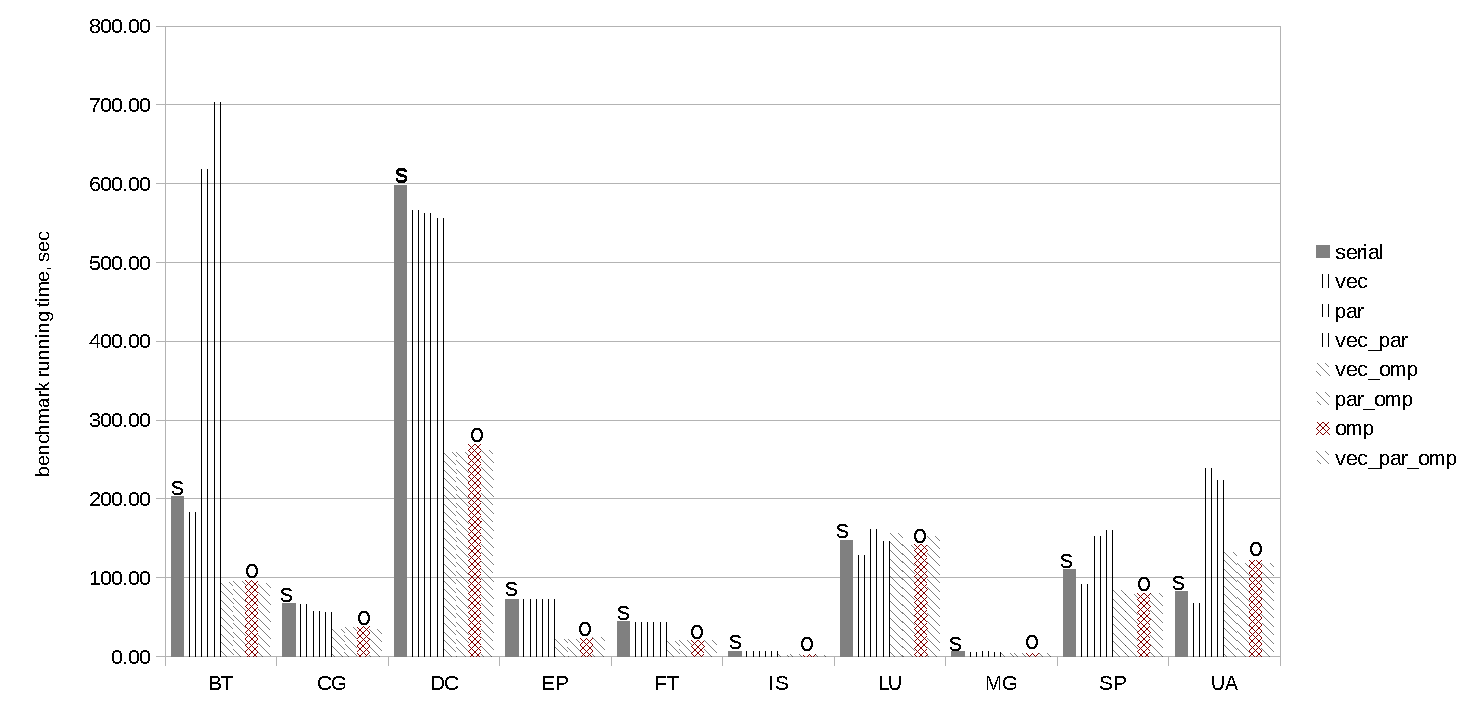
\includegraphics[width=1.0\textwidth]{images/benchmark_runtime.pdf}
\caption{The running time of various NPB benchmarks versions.}
\label{fig:benchmarks_runtime}
\end{figure}

\subsection{Limits of machine learning based methods}
\label{backgrnd_challenges_ml}
\quad Correctness is the most important property of the code. Although important, the running time or any other type of code performance characteristic is not always vitally critical. As all machine learning based techniques have always been characterised by their inherent and ineradicable errors \cite{James:2013:ISL:2517747}, the field of compilers has never been the primary target for these methods. Nonetheless, these techniques have found their application to some problems withing the field.\newline\null
\textit{ML in Compiler Optimization.}
Usually, machine learning based methods target problems, where a misprediction will only lead to a hampered performance and not a functional failure. For example, machine learning based methods have been used for finding the most optimal compiler optimization parameters like predicting the optimal loop unroll factor \cite{4907653,1402082} or determining whether or not a function should be inlined \cite{Zhao2003ToIO,1559966}. These works are supervised classification problems and they target a fixed set of compiler options, by representing the optimization problem as a multi-class classification problem where each compiler option is a class. Recent works try to find a scheduling and optimization of parallel programs for heterogeneous multi-cores. For example, Hayashi \emph{et al.}~\cite{Hayashi:2015:MPH:2807426.2807429} extracts various program features during compilation for use in a supervised learning prediction model aiming at optimality of CPU vs. GPU selection. Evolutionary algorithms like generic search are often used to explore a large design space. Prior works~\cite{Almagor:2004:FEC:997163.997196,Cooper:2005:AAC:1065910.1065921,Ashouri:2017:MMC:3132652.3124452} have used evolutionary algorithms to solve the phase ordering problem (i.e.\ in which order a set of compiler transformations should be applied).\newline\null
\textit{Machine Learning and Parallelization.}
Application of machine learning based methods to the problem of software parallelization has not yet found a widespread practical utility. Mispredictions regarding the code parallelizability can lead to a broken dependency property and thus incorrect program execution. Nonetheless, there have already been works on prediciting loop parallelizability, like the approach of Fried \emph{et al.}~\cite{fried_ea:2013:icmla}. Fried \emph{et al.} train a supervised learning algorithm on code hand-annotated with OpenMP parallelization directives in order to create a loop parallelizability predictor. These directives approximate the parallelization that might be produced by a human expert. Fried \emph{et al.}~focus on the comparative performance of different ML algorithms and studies the predictive performance that can be achieved on the problem and does not produce any practical application.\newline\null
\textbf{\quad In Chapter \ref{assistant} we describe a practical ML based loop parallelization assistant \cite{assistant-aiseps}. Contrary to Fried \emph{et al.}~\cite{fried_ea:2013:icmla} it uses static source code features. Moreover, we use a richer training set, which is not limited to OpenMP pragmas only, but additionally takes the information from the Intel C/C++ Compiler. While Fried \emph{et al.}~focus on the comparative performance of different ML algorithms and study the possibility to learn loop parallelizability property, we do the same, but additionally we contribute a practical assistant capable of ranking loop candidates in their order of merit.}

\section{Data-Centric Parallelization (DCP) problem}
\label{background_dcp}
\subsection{The problem}
\label{background_dcp_problem}
\quad The problem of data-centric parallelization (DCP) is the central motivation for the concept of computational frameworks we propose in Chapter \ref{frameworks}. As it has already been stated the problem of software parallelization is multifaceted. There is a vast range of lower level technical issues, which can turn a perfectly parallelizable at a higher level computation into a non-parallelizable implementation. For example, in Section \ref{background_challenges_automatic} we showed that the main reasons of Intel Compiler failures on SNU NPB benchmarks are alias analysis conservativeness, uninlined function calls and statically unresolvable dependencies. These reasons do not close the set of all possible parallel algorithm implementation failures. Listings \ref{lst:array} and \ref{lst:list} clearly illustrate a yet another potential implementation failure.\newline\null
\begin{minipage}[t]{0.5\linewidth}
\begin{lstlisting}[caption={\raggedright Parallelisable loop operating on a \textbf{linear array}.},label={lst:array},language=C]
for (int i=0; i<1024; i++) {
  a[i]=a[i]+1;
}
\end{lstlisting}
\end{minipage}
%
\begin{minipage}[t]{0.5\linewidth}
\begin{lstlisting}[caption={\raggedright Non-parallelisable loop operating on a \textbf{linked-list}.},label={lst:list},language=C]
for (p=list; p!=NULL; p=p->next) {
  p->value+=1;
}
\end{lstlisting}
\end{minipage}

\quad The above code snippets present two alternative implementations of the same simple and embarrassingly parallel computation. We increment all sequence elements by one. Listing \ref{lst:array} implements the sequence with a regular array linearly laid out in the memory. Listing \ref{lst:list} chooses a linked list as an implementing data structure. While in an array based implementation the compiler knows all element addresses statically and can generate parallel code in advance in the linked list based implementation element addresses can be resolved only dynamically, which leads to a source code non-parallelizability.\newline\null
\quad The data-centric parallelization problem is how to automatically recognise what kind of a data structure is used in the code: is it a tree, a linked-list or a directed acyclic graph? The DCP problem is not solved yet. Automatic methods are limited to relatively simple code bases such as libraries of well known data structures. The most successful methods rely on dynamic analysis of memory graphs. Static techniques such as shape analysis are undecidable and highly conservative and might not finish in a reasonable time for the real software projects. The next section gives a comprehensive literature review on the topic.
\subsection{Literature review}
\label{background_dcp_literature_review}
\quad The idea of automatic discovery of higher level entities in programs is not a new one. This discovery problem is closely interlinked and entangled with alias analysis techniques \cite{Muchnick:1998:ACD:286076} like points-to analysis \cite{Emami:1994:CIP:178243.178264}. Points-to analysis is a variation on data flow analysis techniques. The final output is the sets of pairs of the form (\textit{p}, \textit{x}) (pointer variable \textit{p} points to a stack allocated variable \textit{x}). These techniques are aimed at getting aliasing information regarding stack-allocated pointers.\newline\null
\quad The problem of understanding heap-directed pointers and heap-allocated linked data structures these pointers might point to is addressed with a family of static analysis techniques collectively known as shape analysis. Shape analysis techniques can be used to verify properties of dynamically allocated data structures in compile time. These are among the oldest and most well known techniques. Three-valued logic \cite{Sagiv:1999:PSA:292540.292552}\cite{Wilhelm:2000:SA:647476.760384} can be used as an example. The technique proposes a construction of a mathematical model consisting of logical predicate expressions. The latter correspond to certain pointer operating imperative language program statements. Abstract interpretation of these statements leads to a construction of sets of shape graphs at various program points. Shape graphs approximate the possible states of heap-allocated linked data structures and answer the questions such as node reachability, data structure disjointness, cyclicity, etc. The major limitation of these simplified mathematical models is the lack of precision high level of abstraction leads to. The problem of precise shape analysis is provably undecidable.\newline\null
\quad The work of \cite{Ghiya:1996:TDC:237721.237724} proposes a simplified and hence more practical implementation of shape analysis. Authors propose to use direction \textit{D} and interference \textit{I} matrices instead of complex mathematical models in order to derive shape information on heap allocated data structures. The entry of direction matrix \textit{D[p,q]} says if there exists a path from a node referred to by \textit{p} to a node referred to by q. In other words, if we can enter a path withing the data structure through \textit{p} and exit through \textit{q}. The entry of interference matrix \textit{I[p,q]} says if the paths started from \textit{p} and \textit{q} are going to intersect at some point. Authors implement their technique withing McCAT compiler, which uses SIMPLE intermediate representation with a total of 8 statements (\textit{malloc()}, pointer assignments \textit{p=q}, structure updates \textit{p-$>$next=q}), which are capable of changing \textit{D} and \textit{I} matrices. Statements generate and kill entries in matrices. Moreover, they are capable of changing \textit{Shape} attribute of pointers. The technique has been assessed on various benchmarks (bintree, xref, chomp, assembler, loader, sparse, etc.) from the era before the standard benchmark suites became available. The technique mostly reported shapes as \textit{Trees} (be it a binary tree or a linked-list) or sometimes as \textit{DAGs} or \textit{Cycles} but with higher error rates in these last cases. The latter shows that the technique is imprecise and conservative.\newline\null
\quad One of the more recent techniques designed and developed by Ginsbach et al. is based on the pattern matching on LLVM IR level. The main idea is to specify computational idioms to be recognized in a domain specific constraint based programming language CAnDL \cite{Ginsbach:2018:CDS:3178372.3179515}. Constraints are specified over LLVM IR entities such as instructions, basic blocks, functions, etc. The CAnDL language allows for a rapid prototyping of new compiler optimisations based on pattern recognition and its substitution with an optimised versions of matched idioms. The language and its relatively fast backtracking constraint solver are capable of recognizing not only simple arithmetic idioms (thus performing different peephole optimizations), but more complex computations like general reductions and histograms \cite{Ginsbach:2017:DEG:3049832.3049862}, vector products in graphics shaders \cite{Ginsbach:2018:AML:3296957.3173182}, sparse and dense linear algebra computations and stencils \cite{Ginsbach:2018:AML:3296957.3173182}. Having recognized these computational idioms the work \cite{Ginsbach:2018:AML:3296957.3173182} replaces them with a code for various heterogeneous APIs (MKL, libSPMV, Halide, clBLAS, CLBlast, Lift) and compares the resulting performance demonstrating an improvement over sequential versions and matching performance to a hand-written parallel versions. The technique has been deployed on the sequential C versions of SNU NPB, the C versions of Parboil and the OpenMP C/C++ versions of Rodinia demonstrating improved detection capabilities over the state-of-the-art techniques.\newline\null
\quad The other principally different technique has been recently proposed by Changhee Jung and Nathan Clark \cite{1669122}. The authors developed a Data-structure Detection Tool (DDT) based on the LLVM framework. The tool instruments loads, stores and calls withing program binaries and gathers dynamic traces for sample inputs. The traces are used to recreate a memory allocation graph for program data structures. Call graphs are used to identify interface functions interacting with the built memory graph. DDT traces memory graph properties (number of nodes, edges, etc.) before and after interface function calls into another Daikon tool to compute dynamic invariants (the number of nodes in a memory graph decreses by 1 after every \textit(delete()) interface method call, etc.). At the end manually constructed decision tree is used to probabilistically match observed behavioral patterns against known data structure invariant properties. The technique has been deployed to recognise data structure implementations withing standard libraries like STL, Apache (STDCXX), Borland (STLport), GLib, Trimaran achieving almost perfect recognition accuracy. Moreover, the technique has been able to recognise linked lists in Em3d and Bh Olden benchmarks, along with red-black trees implementing vectors in the Xalancbmk benchmark.\newline\null
\quad There has recently been other published works on the application of dynamic techniques to the problem of dynamic data structure recognition \cite{Rupprecht:2017:DID:3155562.3155607}\cite{Haller:2016:SDS:2938006.2938029}. The technique used in the DDT tool \cite{1669122} makes an assumption, that all modifications and interactions with memory graphs representing data structures happen through a set of interface functions. That is not true, when we deal with aggressively optimising compilers, which may eliminate some code or inline some functions. The MemPick tool \cite{Haller:2016:SDS:2938006.2938029} searches data structures directly on a built dynamic memory graph by analyzing its shape. The graph is built with the help of Intel Pin binary instrumentation tool during quiescent periods, when pointer operations are absent. DSIbin tool \cite{Rupprecht:2017:DID:3155562.3155607} operates with the source code rather than program binaries. Instead of memory points-to graphs it uses strands as primitives, which abstract such entities as singly-linked lists.\newline\null
\quad The work of Dekker \cite{Dekker:1994:ADS:3107859.3107876} addresses software design recovery problem in a completely different way. Contrary to the approaches described above, which operate on the IR and dynamic instruction stream levels, work of Dekker operates at the level of abstract syntax tree. Dekker's tool tries to compact the tree down to a recognizable syntactic patterns by transforming it in accordance to a special grammar.

\section{Imperative and functional programming}
\label{backgrnd_programming_paradigms}
\quad Programming languages can be classified by different \textit{programming paradigms} they support. Among the most general classifications are \textit{imperative} and \textit{declarative} programming languages.\newline\null
\quad Imperative programs are written in a form of instruction sequences, which read and write the \textit{state} of a program. The concept of state is the main characteristic of imperative programming paradigm. Instruction sequences can be structured in various ways. In \textit{procedural programming} paradigm instructions are grouped inside procedures and functions. In \textit{object-oriented programming (OOP)} paradigm instructions are grouped with the data they operate on inside objects of various types or classes. Programs are built either out of various procedures calling each other and exchanging the data or on the interaction of objects of various types. Imperative programs specify the exact sequence of steps to take in order to compute the final result.\newline\null
\quad Declarative programs do not specify the exact sequence of steps and state updates a program needs to do in order to get the desired result. Declarative programs declare the properties of the desired result. The properties can be specified as a set of constraints like in \textit{constraint programming} or a set of linear inequalities like in \textit{linear programming}. \textit{Functional} programming is another subtype of declarative programming. In functional programming the final result is specified as a sequence of stateless function evaluations, which form a tree of expressions. Among the most common constituents are functions like \textit{map}, \textit{reduce}, \textit{fold}, etc. Functions can be passed as arguments and returned from other functions ultimately composing bigger programs.\newline\null
\quad Functional programming is sometimes treated as synonymous with purely functional programming, a subset of functional programming which treats all functions as deterministic mathematical functions, or pure functions. When a pure function is called with some given arguments, it will always return the same result, and cannot be affected by any mutable state or other side effects. This is in contrast with impure procedures, common in imperative programming, which can have side effects (such as modifying the program's state or taking input from a user). Proponents of purely functional programming claim that by restricting side effects, programs can have fewer bugs, be easier to debug and test, and be more suited to formal verification.\newline\null
\quad There are no universally optimal programming paradigms and languages. Some languages are more convenient and suitable for one sort of problem, some languages are better at tackling other problems. For example, functional languages are more convenient in addressing certain domains such as R for statistics and financial analysis. Imperative languages are certainly better for simulations and other state based scientific computations. For that reason, major languages are often multi-paradigm to cover a potentially larger set of problems. Largely imperative C++ language included support for functional programming with its newer standards starting from C++11.\newline\null
\quad \textbf{There is still an unfilled gap between functional and imperative programming paradigms: some problems contain computations, which are better expressed with standard functional concepts (like \textit{maps}, \textit{folds}, \textit{reductions}, etc.), but at the same time require some state keeping. These problems lie at the boundary of functional and imperative programming. In Chapter \ref{frameworks} we propose an idea of \textit{computational frameworks}, which fills that gap. Moreover, we develop a prototype library \cite{frameworks-repo} with a modern and convenient programmer interface, which takes the best features of both object-oriented and functional paradigms and reflects the core ideas behind the concept of computational frameworks.}
\section{OOP and software design patterns}
\label{background_oop_design}
\subsection{Object-Oriented Programming (OOP)}
\label{background_oop}
\quad \textit{Object-oriented programming (OOP)} is arguably the most widely used programming paradigm nowadays. It is supported by almost all major programming languages. At the very essence, in OOP computer programs are designed by making them out of objects that interact with one another. Object interactions are very close to human level of reasoning and logic and thus the paradigm fits quite naturally to a human developer.\newline\null
\quad Objects are instances of different types or classes in OOP terminology. Classes are object specifications. They specify the data objects contain (like an integer \textit{age} field for an object of class \textit{Person}) and the methods used to operate on the data. Classes define the public part of objects as well as their internal implementation. Object-oriented (OO) languages provide a rich set of facilities and features to build programs.\newline\null
\quad \textit{Encapsulation} is used for protection against object misuse and unintended outside interference: data and methods concerned with internal workings are declared \textit{private}, while those designed to form an outward appearance are declared \textit{public}. This facilitates code refactoring, for example allowing the author of the class to change how objects of that class represent their data internally without changing any external code. It also eases debugging by better localizing functionality and thus possible bugs.\newline\null
\quad \textit{Dynamic dispatch} is the responsibility of the object, not any external code, to select the procedure to execute in response to a method call, typically by looking up the method at run time in a table associated with the object. This feature allows a programmer to write general code, which works with abstract interface methods and leave the exact method resolution to be made during the running time of a program.\newline\null
\quad Dynamic dispatch is closely related to the technique of \textit{inheritance}. Inheritance allows classes to be arranged in a hierarchy that represents "is-a-type-of" relationships. Inheritance can be of two types: interface and implementation inheritance. The first one allows a parent class to require its descendants to stick to the same interface. A common interface allows the objects of different classes from the same hierarchy to be operated on by the same type agnostic code. The latter is called a \textit{polymorphism}. The user code can be more concise and abstract. The call of the same method on the parent class or one of its descendants can result into a varying behaviour.\newline\null
\quad Features that are described above do not close the set of all available OOP techniques and mechanisms. These are just the main features we rely on in our project of computational frameworks and are the most important to know.
\subsection{Software design patterns}
\label{background_design}
\quad The presence of all above features makes OOP languages extremely rich with various facilities. That creates a vast design space for software architects and turns the OOP software design into an art. \textit{Software design patterns} \cite{gang-of-four} are reusable solutions to common design problems in OOP. Design patterns have been well tested and are proven to be the most reliable and elegant solutions for design problems they target.\newline\null
\quad Design patterns live at an intermediate level between the exact algorithm and a programming paradigm and are language agnostic. Design patterns specify and document solutions to common design problems. These solutions consist of a set of classes, objects and the ways they interact with one another. It is agreed to classify patterns into 4 distinct categories: creational, structural, behavioural and concurrency patterns. Here we are going to mention only those patterns, which are the most relevant to our project of computational frameworks.\newline\null
\quad The \textit{command} pattern is a behavioural pattern, where a command object is used to encapsulate all the information needed to perform an action or trigger some event at a later time. The other participants are the receiver, invoker and client. The central ideas of this design pattern closely mirror the semantics of first-class functions and higher-order functions in functional programming languages. Specifically, the invoker object is a higher-order function of which the command object is a first-class argument.\newline\null
\quad One can see the command pattern used in combination with the \textit{chain of responsibility pattern}, which is a design pattern consisting of a source of command objects and a series of processing objects. Each processing object contains logic that defines the types of command objects that it can handle; the rest are passed to the next processing object in the chain. In a variation of the standard chain of responsibility model, some handlers may act as dispatchers, capable of sending commands out in a variety of directions, forming a \textit{tree of responsibility}. The chain of responsibility pattern promotes the idea of \textit{loose coupling}, where the system consists of multiple components, which know little or nothing about the definitions of other components.\newline\null
\quad Another very relevant pattern is a \textit{template method} pattern. The template method is a method in a superclass, usually an abstract superclass, and defines the skeleton of an operation in terms of a number of high-level steps. These steps are themselves implemented by additional helper methods in the same class as the template method. The helper methods may be either abstract methods, for which case subclasses are required to provide concrete implementations, or hook methods, which have empty bodies in the superclass. Subclasses can (but are not required to) customize the operation by overriding the hook methods. The intent of the template method is to define the overall structure of the operation, while allowing subclasses to refine, or redefine, certain steps.\newline\null
\quad The \textit{visitor} pattern is a way of separating an algorithm from an object structure on which it operates. A practical result of this separation is the ability to add new operations to existing object structures without modifying the structures. In essence, the visitor allows adding new virtual functions to a family of classes, without modifying the classes. Instead, a visitor class is created that implements all of the appropriate specializations of the virtual function. The visitor takes the instance reference as input, and implements the goal through double dispatch.\newline\null
\quad Software design patterns can be more down to the language like the \textit{curiously recurring template pattern (CRTP)}, which is an idiom in C++ where a class X derives from a class template instantiation using X itself as template argument.\newline\null
\quad \textit{Software design patterns} specify and document the best practices to solve various commonly reoccurring problems. At the end it is the experience, mastery and ingenuity of a programmer which determine the final software design.  

\subsection{Computational frameworks and design patterns}
\label{background_design_frameworks}
\quad When we introduce the concept of computational frameworks, it is very important to mention software design patterns. While not exactly the same, the two concepts have an overlap. Computational frameworks do not specify the exact algorithms and data structures that must be used to implement the task, but alike declarative programming rather define the requirements on a higher level computation. For instance, a fractal can be implemented as a tree or as a heap and a fold can be implemented with an array or with a linked list, but the higher order computational requirements must be met. One can see a similarity to the template method design pattern, which also specifies the main computation and leaves some lower level steps to be defined by a user. One can see a similarity between the chain of responsibility pattern and the fold computational framework. The latter is also a visitor pattern in its own way. While the backbone computation of our frameworks is implemented with a template method pattern, the command pattern is used to specify the user defined custom part. Computational frameworks also promote the idea of loose coupling by keeping the computational procedure strictly decoupled from the side effects accumulation.\newline\null
\textbf{\quad Computational frameworks embody the best ideas of all relevant software design patterns (template method, command, curiously recurring template pattern, etc.) and can be also considered as such. They relieve a programmer from a complex task of software architecture design by providing a ready solutions with all computational, communicational and data access patterns known and implemented in advance.}
\section{Parallel algorithmic skeletons}
\label{backgrnd_skeletons}
\quad Algorithmic skeletons or parallelism patterns \cite{mccool-patterns} are a high-level parallel programming model, that take advantage of common programming patterns to hide the complexity of parallel and distributed applications. For example, the basic algorithmic skeletons are \textit{map}, \textit{pipeline}, \textit{reduce}, \textit{scan}, \textit{stencil}, \textit{divide and conquer}, \textit{task farm}, etc. More complex parallelism patterns can be composed out the basic ones. When the computational and data access patterns are known in advance, algorithmic skeletons hide all complexities (synchronization, communication, etc.) of parallel programming and let a user to concentrate on the algorithmic part. Algorithmic skeletons are higher than other parallel programming models like MPI, OpenMP, POSIX threads and they have a vast array of various implementations and libraries. The latter vary by the programming language they target, distribution library used to implement parallel/distributed computations internally (like MPI, OpenMP, etc.), the sets of supported skeletons and the allowed level and way of skeleton nesting, i.e composing a more complex patterns out the basic ones.\newline\null
\textbf{\quad While algorithmic skeletons or parallelism patterns stress an algorithmic component of the computation, computational frameworks contain an underlying data structure that might accumulate computation's side effects.}
\section{Benchmark studies}
\label{background_benchmarks}
\quad In our projects we used three benchmark suites. We trained our machine learning (ML) based loop parallelization assistant \cite{assistant-aiseps} (see Chapter \ref{assistant}) with Seoul National University's implementation \cite{snu-npb-benchmarks} of the NASA Parallel Benchmarks (NPB) \cite{snu-npb-benchmarks}. The suite comes in two versions: sequential and parallelized with OpenMP. We used the latter to extract ML training labels. Moreover, the suite contains a load of various sorts of parallel loops, which makes it a good training set. For the data-centric parallelization (DCP) project we started with the SPEC CPU2006 benchmarks. The complexity level of that suite and the perspective we derived from the suite study led us to a simpler suite of Olden benchmarks. We used the latter for the project of computational frameworks (see Chapter \ref{frameworks}). Below we provide descriptions of benchmarks, so a reader can develop a better feel for the problems we tackle and the code we work with.
\subsection{NASA Parallel Benchmarks (NPB)}
\label{background_benchmarks_npb}
\quad NAS Parallel Benchmarks (NPB) \cite{nasa-parallel-benchmarks} target performance evaluation of highly parallel supercomputers. NPB are "paper-and-pencil" benchmarks, i.e they do not provide the exact implementation, but rather specify various computational problems at a higher level. There are various implementations. We used the one from Seoul National University (SNU) - SNU NPB \cite{snu-npb-benchmarks}.\newline\null
\quad There are 10 various benchmarks in the suite. Benchmarks perform various scientific computations. They solve various systems of linear equations, compute gradients, work with matrices (compute matrix transpose, inverse, etc.), solve differential equations, solve heat and diffusion equations on the mesh, compute 3d grids, etc. The main data structure used in all SNU NPB benchmarks is a flat multidimensional array. These arrays are processed in loops of various complexity levels including embarrassingly parallel loops like (\textit{a[i] = b[i] + c[i]}), parallel copy and initialization loops (\textit{a[i] = b[i]} and \textit{c[i] = 0.0}), loops computing simple reductions, unrolled loops, multilevel nested loops and loops with uninlined function calls, as well as more complex loops with \textit{if} and \textit{switch} statements and loops with statically unknown iteration numbers and indirect array references (\textit{a[i] = b[c[i]]}).\newline\null
\quad To the biggest part, these benchmarks are inherently parallel, but surprisingly their automatic parallelization with the best state-of-the-art Intel C/C++ Compiler (ICC) \cite{icc-compiler} results into a slowdown (see Section \ref{background_challenges_automatic}). Moreover ICC fails to recognize a lot of parallel loops. Our parallelization assisatant increases parallelization coverage and leads a programmer to achieve a manual expert level parallel benchmark performance faster. 
\subsection{SPEC CPU2006}
\label{background_benchmarks_spec}
\quad The project of Data-Centric Parallelization (DCP) started with the feasibility studies of the SPEC CPU2006 benchmark suite. We studied the feasibility of the automatic data structure recognition techniques on these benchmarks. Although the benchmarks proved to be extremely complex for such techniques, these studies directed our further efforts and ultimately led to the concept of computational frameworks being an inseparable blend of data structures and algorithms. The key lessons we learnt from the SPEC CPU2006 benchmarks are an enormous complexity of the real legacy code and a very close relationship between data structures and algorithms. Let alone automatic techniques, it might take some weeks for an expert engineer to understand what a single benchmark is actually doing. Below we describe some of the benchmarks we looked at.\newline\null
\quad \textbf{429.mcf} \quad The benchmark is derived from MCF, a program used for single-depot vehicle scheduling in public mass transportation. The benchmark operates with a complex network of nodes and arcs linearly allocated on the heap memory. Despite the simplicity of allocation, every node and arc has numerous pointers forming several object linking chains. Pointers are set in different places withing the source code base (during allocation as well as during consecutive network structure updates), making the deduction of the actual data structure shape a task of grand complexity. The network forms a spanning tree with several properties true of its nodes: every node has only one child pointer and if a node has several children, then the latter are connected through sibling pointers starting from the first child.\newline\null
\quad\textbf{The tree data structure presents a high interest from the point of its recognition. But even a manual source code analysis and transformation requires a serious effort. Static automatic techniques seem infeasible, while dynamic ones seem to be a grand challenge.}\newline\null
\quad \textbf{456.hmmer} \quad Searches a DNA sequence database given a Profile Hidden Markov Model (HMM). The benchmark uses the Viterbi algorithm. The implementation works with four dynamic programming matrices allocated linearly as arrays. Algorithm walks either horizontally or diagonally along these matrices and computes reductions of maps. The computation is parallelizable and there has been successful work \cite{Ganesan:2010:AHG:1854776.1854844}\cite{inria} doing it manually for specialized hardware.\newline\null
\quad\textbf{Despite the complexity of its core function \textit{P7Viterbi()}, the benchmark presents a very high interest for the application of our computational frameworks. Reductions of maps perfectly fit the purpose. We view it as a future work.}\newline\null
\quad \textbf{400.perlbench} \quad This benchmark is a cut-down Perl interpreter, which implements the regular expression matching state machine. The benchmark processes the bitcode of a compiled regular expression instruction by instruction. Although, instructions have the same size and are laid out linearly in memory, there might be branches and the whole processing happens in a linked-list offset directed fashion. That requires sequential execution and is far beyond the capabilities of any existent techniques.\newline\null
\quad\textbf{The benchmark is neither parallel nor a simple one. It makes no point to apply any recognition techniques here.}\newline\null
\quad \textbf{470.lbm} \quad The benchmark implements a Lattice Boltzmann Method (LBM) and is a relatively simple one (around ~1400 LOC). The main underlying data structures the benchmark works with are the two 3D grids mapped onto a linear array space, which simulate incompressible fluids in 3D. The benchmark runs over arrays a specified number of time steps. Every array element represents a point from a 3D grid and consists of a number of velocity vector projections at this point. The values of these projections are being combined and mapped in a stencil fashion. The computation is highly parallel.\newline\null
\quad\textbf{The benchmark operates with 3D grids laid out on regular arrays. The latter do not present a great deal of interest from the point of data structure recognition. Although, it would be interesting to try to recognize an algorithmic stencil.}
\subsection{Olden}
\label{background_benchmarks_olden}
\quad Although the studies of SPEC CPU2006 benchmarks have proved their enormous complexity for the task of automatic data structure recognition, we acquired a good perspective and narrowed our research path to a much simpler suite of Olden benchmarks. Computations and algorithmic patterns present in Olden benchmarks have ultimately led us to the concept of \textit{computational frameworks} (see Chapter \ref{frameworks}).\newline\null
\quad Olden benchmark suite consists of 10 benchmarks. For our project we looked at 6 of those (\textit{bisort}, \textit{health}, \textit{perimeter}, \textit{treeadd}, \textit{mst} and \textit{tsp} benchmarks). The nature of different Olden benchmarks varies. Benchmarks health, treeadd and perimeter perform essentially the same computational pattern, but for different problems. We call that pattern a fractal and it is basically a parallel tree growth and processing. Benchmarks tsp and mst solve 2 well-known graph problems namely travelling salesman problem (TSP) and minimum spanning tree (MST) construction. The other 4 benchmarks perform scientific numerical computations and are bigger, more complex and less interesting from the perspective of data structure recognition.\newline\null
\quad \textbf{bisort} \quad \textit{\textbf{Definition} A sorted sequence is a monotonically non-decreasing (or non-increasing) sequence. A bitonic sequence is a sequence with $x_{0} \leq ... \leq x_{k} \geq x_{k+1} \geq ... \geq x_{n} - 1$ for some k, or a circular shift of such a sequence.}\newline\null
\quad The sequence is implemented as a binary tree (recursive calls to the left and right subtrees). The algorithm is based on a sorting comparator network consisting of several layers. The network can be and is implemented in a divide and conquer way similar to that of a well-known merge sort. Sort() function is called on the left and right array halves recursively. The merging step of the merge sort algorithm is substituted with compare-and-swap step. The latter is possible due to input sequences required to be bitonic.\newline\null
\quad\textbf{The benchmark is heavily based on pointers, tree swaps and rotations. It presents an interest from the point of divide and conquer algorithm recognition. Static techniques are unlikely to handle the legacy source code of that complexity and style. Dynamic techniques might be able to see the binary tree.}\newline\null
\quad \textbf{health} \quad The health benchmark fits into the fractal computational framework the best and hence delivers the most promising performance results. Health benchmark does a simulation of the Columbian healthcare system and is based on a complete 4-ary tree of villages. One can view the tree as the hierarchical structure reflecting various levels of municipal divisions: the root is the capital, leaves represent villages and the nodes on intermediate tree levels represent small towns and bigger cities. The closer to the root, the bigger the settlement and higher the level of hospital expertise. Every village has its own hospital. Figure \ref{fig:health_benchmark} illustrates the tree.
\begin{figure}
\centering
\begin{minipage}{.5\textwidth}
  \centering
  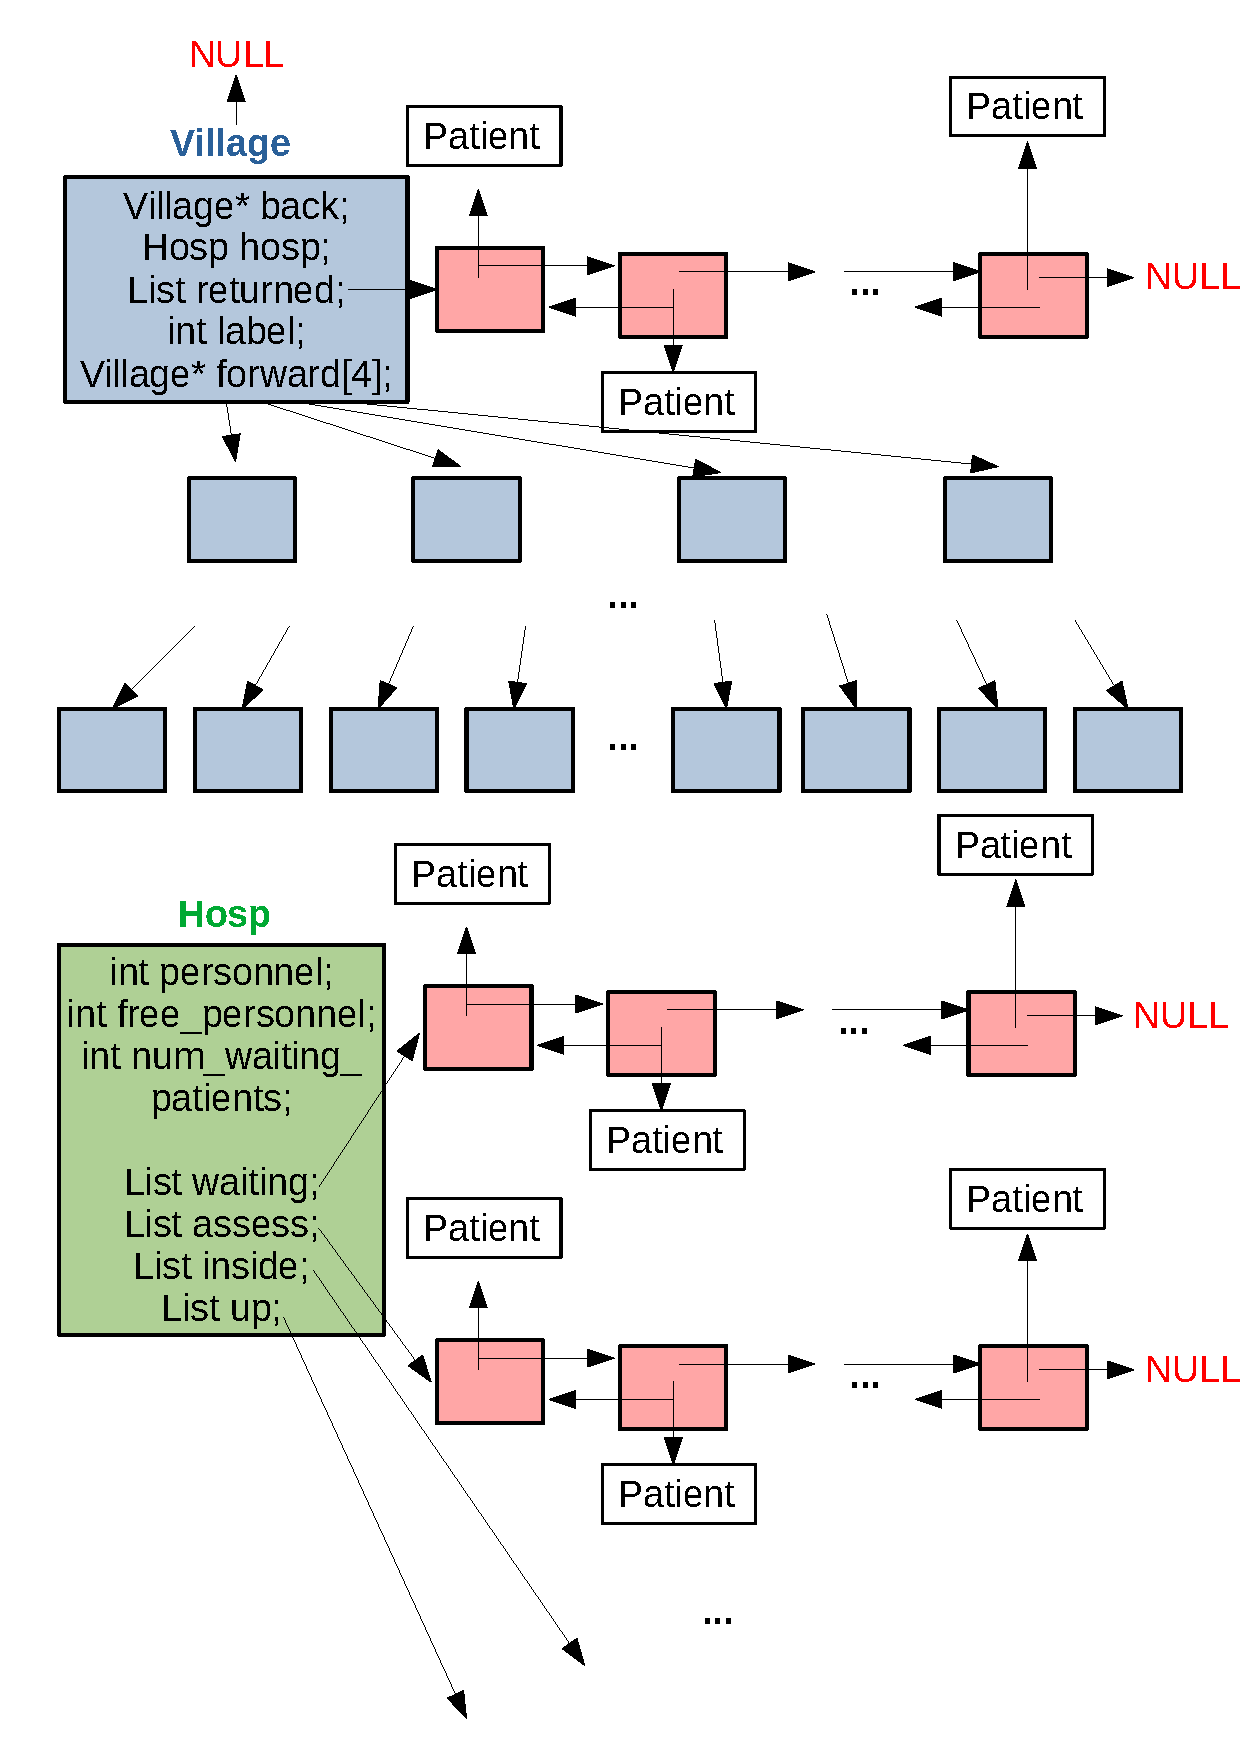
\includegraphics[width=0.9\linewidth]{images/village_tree.pdf}
  \captionof{figure}{The \textit{health} benchmark.}
  \label{fig:health_benchmark}
\end{minipage}%
\begin{minipage}{.5\textwidth}
  \centering
  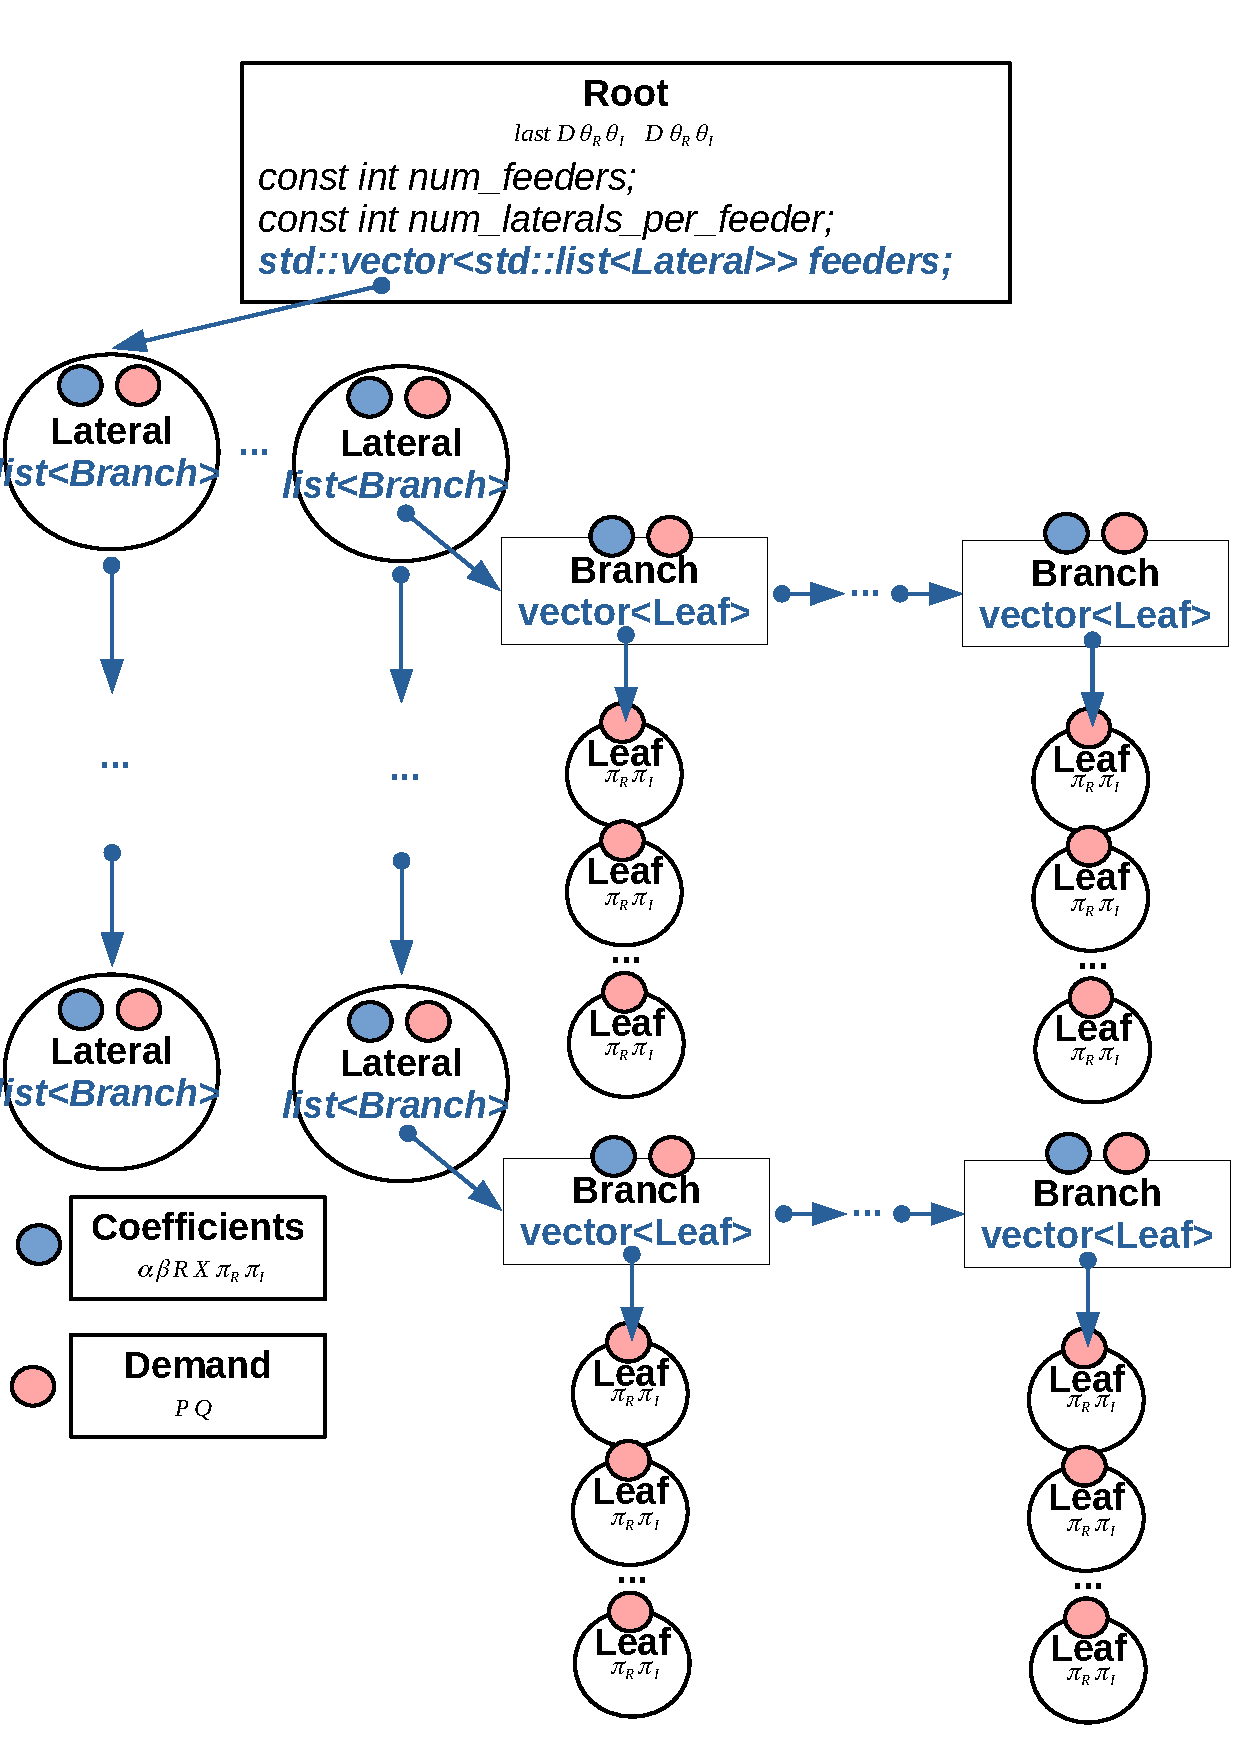
\includegraphics[width=0.9\linewidth]{images/power_scheme.pdf}
  \captionof{figure}{The \textit{power} benchmark.}
  \label{fig:power_benchmark}
\end{minipage}
\end{figure}\newline\null
\quad Simulation starts at the tree root and goes down to the leaves. There are people who fall ill in every village and when they do they go into the local hospital for an assessment and in case they are ill for treatment. If local staff cannot give an accurate diagnosis a patient goes up the tree to a bigger settlement with a higher staff expertise level. As the simulation goes the lists of patients waiting, under assessment or inside the hospital for treatment grow and the benchmark state becomes bigger. So does the workload. The computation is parallel: all tree node child sub-trees can be simulated independently. Child nodes pass lists of patients to their parents and the latter take them to their local hospitals.\newline\null     
\quad \textbf{The benchmark operates with quad tree structures and does it in a highly parallel fashion. In our work we call that pattern a fractal. The latter is a computational framework, i.e. the blend of an algorithm and a data structure. The whole structure can be aimed at for an automatic recognition (not just a separate tree or an algorithmic skeleton, but both) even with static techniques.}\newline\null
\quad \textbf{perimeter} \quad The perimeter benchmark is another example of the fractal framework. The benchmark computes the perimeter of a ring (r=1024, R=2048). Figure \ref{fig:perimeter_benchmark} illustrates the process. The ring is placed onto a square, which is then being continuously and recursively divided into 4 equal sub-squares (southwest, northwest, southeast and northeast). Only guided by the stop condition the process continues further. We divide the square further if it falls on the intersection with the ring boundary. If the square falls completely inside the ring or completely outside we stop the division. Division also stops, when the square area becomes less than a preset granularity (or equivalently the depth of the tree). The process can be represented as a growing unbalanced quad tree. Squares are the nodes of the tree. Squares inside the ring (all 4 square corners $(x,y)$ are $r^{2} < x*x + y*y < R^{2}$) are painted black, while those outside are painted white. In other words, the growth stops at black and white tree nodes and continues for those representing squares on the intersection with the ring. Finally, the resulting grid is being traversed to catch all flips of color. When the flip is detected we increment the perimeter counter by the square area adjacent to the flip boundary. The latter results into the final perimeter approximation.\newline\null
\quad \textbf{The benchmark operates with quad tree structures and does it in a highly parallel fashion. This fits into the fractal pattern as well. The only difference from the health benchmark is the tree growth stop condition resulting into unbalanced tree. Automatic fractal recognition seems harder, but still possible.}
\begin{figure}[ht]
\begin{center}
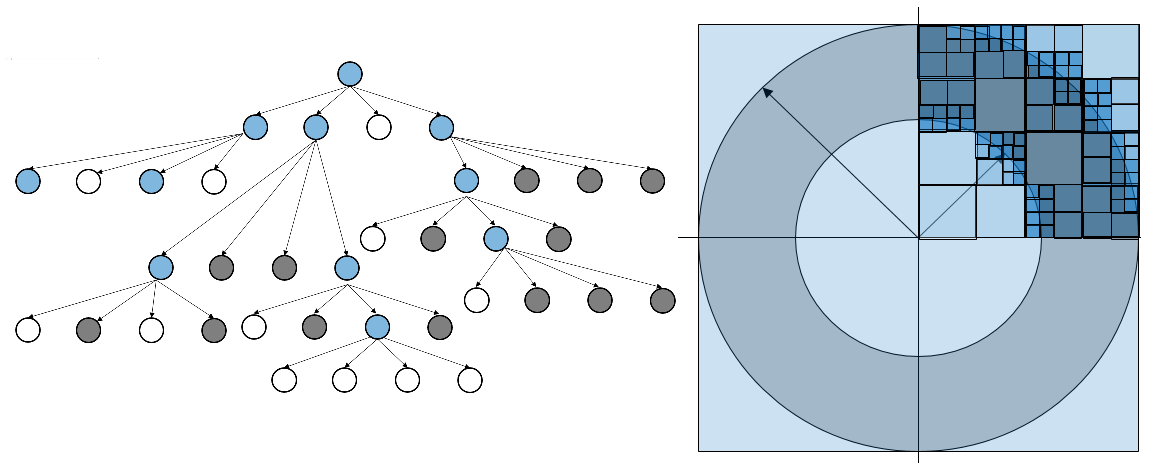
\includegraphics[width=1.0\textwidth]{images/perimeter_benchmark.png}
\caption{The \textbf{perimeter} benchmark. Computational pattern can be represented by an unbalanced quad tree.}
\label{fig:perimeter_benchmark}
\end{center}
\end{figure}\newline\null
\quad \textbf{power} \quad Another key benchmark for us is the power pricing computation benchmark. The benchmark is based on a composite hierarchical structure of C arrays and pointer-based linked lists of various objects: Root, Laterals, Branches and Leaves. Figure \ref{fig:power_benchmark} illustrates the data structure. The algorithm is basically composed of folds and reductions. C arrays are reduced and linked lists are folded. The algorithm works recursively and starts with the Root::compute() call. The method accumulates the power demand
Demand(P,Q) from all lists of Laterals and does a reduction to a final Demand(P,Q) value. Accumulation starts with the end of each lateral list. Each lateral accumulates its power demand from all its branches and the latter in turn accumulate their power demand from all their leaves. The leaves call optimize\_node() method, which does a chunk of scientific computations (gradients, vectors, etc.), which compute P and Q. Finally, Root::compute() is called iteratively from a while loop of power\_pricing\_problem(). Iteration continues up until P and Q error becomes less than the required epsilon. Before every simulation step the benchmark does an injection of coefficients into the structure. Every simulation step leaves computed side effects on the coefficients stored withing various objects.\newline\null
\quad \textbf{The power benchmark operates with sequences and linked lists. Sequences are reduced and linked lists are folded. These patterns correspond to and inspire our Fold and Reduce computational frameworks.}\newline\null
\quad \textbf{treeadd} \quad The treeadd benchmark is a very small and simple one. It does a recursive reduction on a pointer-linked binary tree. To create a workload the reduction is done repetitively inside the loop.\newline\null
\quad \textbf{The treeadd benchmark is a straightforward example of the fractal computational framework. Although, the workload is to small for its effective application.}\newline\null
\paragraph{mst} Minimum Spanning Tree (MST) benchmark does an MST weight computation of a complete graph. Computation is approximate and the algorithm looks like it might finish with incorrect result. Nevertheless, the benchmark can be used for the purpose of computational workload. Graph is represented as a linked list of vertices. Every node in the list has a hash table of incident edges. Graph is complete: each vertex is connected to all other vertices in the graph (except itself). Algorithm repeatedly traverses the list of vertices and gradually accumulates the MST weight. On every traversal algorithm picks the node in the list to use as an input for the next traversal. In that sense, there is a cross iteration/traversal dependency. The code below summarises the benchmark.\newline\null
\begin{minipage}[t]{\linewidth}
\begin{lstlisting}[caption={The main algorithm of mst benchmark.},label={lst:mst_code},language=C]
vertex = list;
list = list->next;
while (num_vertices) {
    ret = traverse_vertex_list(vertex, list);
    mst_weight += ret.distance; // accumulate the final result
    vertex = ret.vertex; // next vertex to measure the distance against
    num_vertices--;
}
return mst_weight;
\end{lstlisting}
\end{minipage}
\paragraph{tsp} Travelling Salesman Problem (TSP). The benchmark generates a set of dots scattered on a 2D plane. Dots represent cities and are specified by their (x,y) coordinates. The TSP problem is to visit all the cities and return to the city of origin having passed the minimal distance. In other words, the algorithm returns a cycled sequence of cities, where proximity of elements in the sequence in terms of order means their spatial proximity on the 2D plane. The algorithm’s work resembles that of an insertion sort. The sequence is divided into 2 parts. Ordered part and unordered part. At first, ordered part consists of just 1 element. On every iteration the algorithm takes the next element out of unordered part, finds it a pairing element inside the ordered part (with the minimal distance between them) and inserts the element into the ordered subsequence next to its pair. At the end we get the sequence with the property that closest dots stand the closest in the sequence. The benchmark is based on a binary tree being transformed into doubly linked list. Every node of the tree represents a city located on 2D plane with randomly generated (x,y) coordinates. The build\_tree() method is written in a way to generate a uniform distribution of dots on the plane.

%